\documentclass[12pt]{article}
\usepackage[T2A]{fontenc}
\usepackage[utf8]{inputenc}
\usepackage{graphics}
\usepackage[english, russian]{babel}
\usepackage{csquotes}
\usepackage{graphicx}
\usepackage{amsmath}
\usepackage{longtable}
\usepackage[left=25mm, top=20mm, right=25mm, bottom=30mm,nohead,nofoot]{geometry}
\usepackage{verbatim}
\usepackage{hyperref}
\usepackage{amssymb,latexsym}  % Standard packages
\usepackage{MnSymbol}
\usepackage{mathrsfs}
\usepackage{amsthm}
\usepackage{indentfirst}
\usepackage[nottoc,numbib]{tocbibind}
\usepackage{float}

\usepackage{listings}
\usepackage{fancyhdr}
\usepackage{multirow}
\usepackage{hhline}
\usepackage{listings}
\usepackage{color}
\usepackage{color,colortbl}
\usepackage{epigraph} %%% to make inspirational quotes.
\usepackage[all]{xy} %for XyPic'a
\usepackage{color} 
\usepackage{amscd} %для коммутативных диграмм
\usepackage{url}
\usepackage{breakurl}
\usepackage[titles]{tocloft}

%******************************************************************
%******************************************************************

\setcounter{tocdepth}{4}
\graphicspath{ {./pic/} }

\begin{document}

\begin{titlepage}
	\center
		Санкт-Петербургский Политехнический 
		университет Петра Великого
		Институт прикладной математики и механики
		\\ \textbf{Кафедра «Прикладная математика»}

	\vfill ~
	\textbf{
		\\ \large ЛАБОРАТОРНАЯ РАБОТА №5
	}
	\\	по дисциплине 
	\\	"Математическая статистика"

	\vfill ~

	Выполнил студент гр. \textbf{33631/1} \\
	\textbf{Лансков.Н.В.} \\ 

\vfill

{\large}	Санкт-Петербург
\\ 2019
\end{titlepage}

%%%
% Table of conetnts 
%%%
% \settocdepth{chapter}
\tableofcontents
\newpage
% \listoffigures
% \newpage
\listoftables
\newpage
\pagebreak

% \setcounter{chapter}{1}

%%%
% Text
%%%
\section{Постановка задачи}
Необходимо построить выборки объёмом $20, 60, 100, 1000$ для двумерного нормального распределения с коэффициентами корреляции $\rho = 0, 0.5, 0.9$

Вычислить коэффициент корреляции Пирсона, Спирмана и квадрантный коэффициент корреляции для каждой выборки. Эти же вычисления повторить для смеси двумерных нормальных распределений \cite{mix}: 
\begin{equation}
    f(x,y) = 0.9N(x,y,0,0,1,1,0.9)+0.1N(x,y,0,0,10,10,-0.9)
\end{equation}
На графике изобразить точки выборки и эллипс равновероятности.

\section{Теория}

\begin{enumerate}
    \item Двумерное нормально распределение \cite{5_1}:
        \begin{equation}
        N(x,y,0,0,1,1,\rho) = \frac{1}{2\pi\sqrt{1-\rho^2}}e^{-\frac{1}{2(1-\rho^2)}(x^2-2\rho x y+y^2)} \label{dnd}
        \end{equation}
    
    \item Коэффициент корреляции Пирсона \cite{5_2}:
        \begin{equation}
        r_{xy} = \left(\sum\limits_{i=1}^n(x_i-\overline{x})(y_i-\overline{y})\right)\left(\sum\limits_{i=1}^n(x_i-\overline{x})^2\sum\limits_{i=1}^n(y_i-\overline{y})^2\right)^{-\frac{1}{2}} \label{ccp}
        \end{equation}
    \item Коэффициент корреляции Спирмана \cite{5_3}:
        \begin{equation}
        \rho_n = 1 -  \frac{6}{n^3-n}\sum\limits_{i=1}^n d_i^2\label{ccs}
        \end{equation}
        
    \item Квадрантный коэффициент корреляции \cite{5_4}:
        \begin{equation}
        \overset{\wedge}{q} = \frac{1}{n}\sum\limits_{i=1}^n sign(x_i-med\;x)sign(y_i-med\;y)\label{qcc}
        \end{equation}
\end{enumerate}

\section{Реализация}
Работы была выполнена на языке $Python 3.7.$
Для генерации выборок использовался модуль \cite{numpy}.
Для построения графиков использовалась библиотека matplotlib \cite{plotlib}.
Функции распределения обрабатывались при помощи библиотеки scipy.stats \cite{skp}

\section{Результаты}

\begin{figure}[H]
    \centering
    \caption{Графики двумерного нормального распределения\eqref{dnd} при $p=0.0$ }
    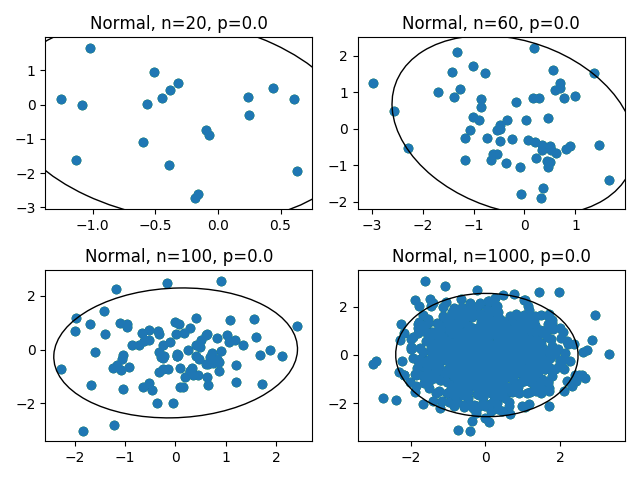
\includegraphics[scale = 0.6]{p00.png} 
    \label{fig:dis_norm_gis0}
\end{figure}
\begin{table}[H]
\caption{Результаты для двумерного нормального распределения \eqref{dnd} при $p=0.0$}
\label{tab:my_label1}
\begin{center}
\vspace{5mm}
\begin{tabular}{|c|c|c|c|c|c|c|c|c|}
\hhline{----~----}
\multicolumn{4}{|c|}{Normal  $n=20,\;  p=0.0$} &\multirow{11}{*}{$\cdot$} & \multicolumn{4}{c|} {Normal  $n=60,\;  p=0.0$}
\\
\hhline{----~----}
&Pearson     &Spearman    &Quad &   & & Pearson     &Spearman    &Quad        \\    
\hhline{----~----}
		E   &-0.05816&-0.07609&-0.10000&  &E   &0.01971&0.01170&0.00000\\
\hhline{----~----}
		$E^2$ &0.07798&0.08066&0.06000&  &$E^2$ &0.01806&0.01560&0.00978\\
\hhline{----~----}
		D   &0.07460&0.07487&0.05000&  &D   &0.01767&0.01546&0.00978\\\rowcolor{codegray}
\hhline{----~----} 
\multicolumn{9}{c}{}\\
\hhline{----~----}
\multicolumn{4}{|c|}{Normal  $n=100,\;  p=0.0$} & & \multicolumn{4}{c|}{Normal  $n=1000,\;  p=0.0$}\\
\hhline{----~----}
&Pearson     &Spearman    &Quad&  & &Pearson     &Spearman    &Quad     \\
\hhline{----~----}
		E   &0.01742&0.00400&0.01200& &E   &0.00909&0.00753&0.00360\\
\hhline{----~----}
		$E^2$ &0.00723&0.00366&0.00272& &$E^2$ &0.00172&0.00146&0.00076\\
\hhline{----~----}
		D   &0.00693&0.00365&0.00258& &D   &0.00163&0.00140&0.00074\\
\hhline{----~----}
\end{tabular}
\end{center}
\end{table}




\vspace{-1cm}
\begin{figure}[H]
    \centering
    \caption{Графики двумерного нормального распределения\eqref{dnd} при $p=0.5$ }
    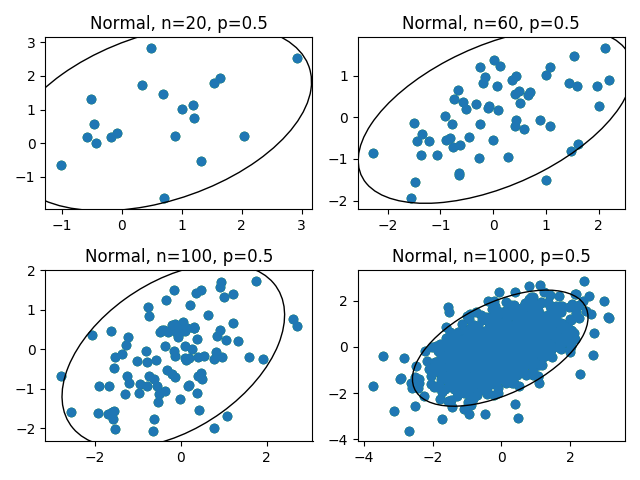
\includegraphics[scale = 0.6]{p05.png}
    \label{fig:dis_norm_gis1}
\end{figure}
\begin{table}[H]
\caption{Результаты для двумерного нормального распределения \eqref{dnd} при $p=0.5$}
\label{tab:my_label2}
\begin{center}
\vspace{5mm}
\begin{tabular}{|c|c|c|c|c|c|c|c|c|}
\hhline{----~----}
\multicolumn{4}{|c|}{Normal  $n=20,\;  p=0.5$} &\multirow{11}{*}{$\cdot$} & \multicolumn{4}{c|} {Normal  $n=60,\;  p=0.5$}
\\
\hhline{----~----}
&Pearson     &Spearman    &Quad &   & & Pearson     &Spearman    &Quad        \\    
\hhline{----~----}
		E   &0.51442&0.45579&0.36000&  &E   &0.55504&0.52874&0.34000\\
\hhline{----~----}
		$E^2$ &0.27969&0.23585&0.16000&  &$E^2$ &0.31584&0.29272&0.12756\\
\hhline{----~----}
		D   &0.01506&0.02811&0.03040&  &D   &0.00777&0.01315&0.01196\\\rowcolor{codegray}
\hhline{----~----} 
\multicolumn{9}{c}{}\\
\hhline{----~----}
\multicolumn{4}{|c|}{Normal  $n=100,\;  p=0.5$} & & \multicolumn{4}{c|}{Normal  $n=1000,\;  p=0.5$}\\
\hhline{----~----}
&Pearson     &Spearman    &Quad&  & &Pearson     &Spearman    &Quad     \\
\hhline{----~----}
		E   &0.48316&0.47127&0.28800& &E   &0.51152&0.49627&0.34560\\
\hhline{----~----}
		$E^2$ &0.23773&0.22671&0.09952& &$E^2$ &0.26231&0.24699&0.11993\\
\hhline{----~----}
		D   &0.00429&0.00461&0.01658& &D   &0.00066&0.00070&0.00049\\
\hhline{----~----}
\end{tabular}
\end{center}
\end{table}



\vspace{-1cm}
\begin{figure}[H]
    \centering
    \caption{График двумерного нормального распределения \eqref{dnd} при $p=0.9$ }
    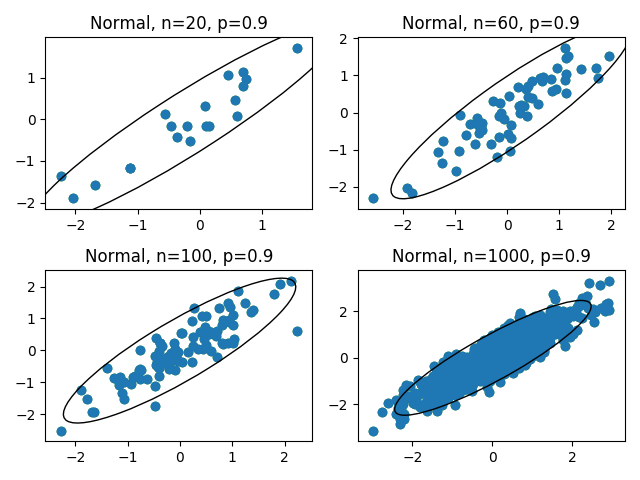
\includegraphics[scale = 0.6]{p09.png} 
    \label{fig:dis_norm_gis2}
\end{figure}
\begin{table}[H]
\caption{Результаты для двумерного нормального распределения \eqref{dnd} при $p=0.9$}
\label{tab:my_label3}
\begin{center}
\vspace{5mm}
\begin{tabular}{|c|c|c|c|c|c|c|c|c|}
\hhline{----~----}
\multicolumn{4}{|c|}{Normal  $n=20,\;  p=0.9$} &\multirow{11}{*}{$\cdot$} & \multicolumn{4}{c|} {Normal  $n=60,\;  p=0.9$}
\\
\hhline{----~----}
&Pearson     &Spearman    &Quad &   & & Pearson     &Spearman    &Quad        \\    
\hhline{----~----}
		E   &0.89459&0.85218&0.58000&  &E   &0.90863&0.89374&0.76667\\
\hhline{----~----}
		$E^2$ &0.80225&0.72999&0.37200&  &$E^2$ &0.82605&0.80025&0.59689\\
\hhline{----~----}
		D   &0.00196&0.00378&0.03560&  &D   &0.00044&0.00147&0.00911\\\rowcolor{codegray}
\hhline{----~----} 
\multicolumn{9}{c}{}\\
\hhline{----~----}
\multicolumn{4}{|c|}{Normal  $n=100,\;  p=0.9$} & & \multicolumn{4}{c|}{Normal  $n=1000,\;  p=0.9$}\\
\hhline{----~----}
&Pearson     &Spearman    &Quad&  & &Pearson     &Spearman    &Quad     \\
\hhline{----~----}
		E   &0.90133&0.89249&0.72800& &E   &0.89728&0.88880&0.71800\\
\hhline{----~----}
		$E^2$ &0.81259&0.79674&0.53248& &$E^2$ &0.80514&0.79000&0.51568\\
\hhline{----~----}
		D   &0.00019&0.00021&0.00250& &D   &0.00004&0.00004&0.00015\\
\hhline{----~----}
\end{tabular}
\end{center}
\end{table}





\vspace{-1cm}
\begin{figure}[H]
    \centering
    \caption{Графики смеси двумерных нормальных распределений }
    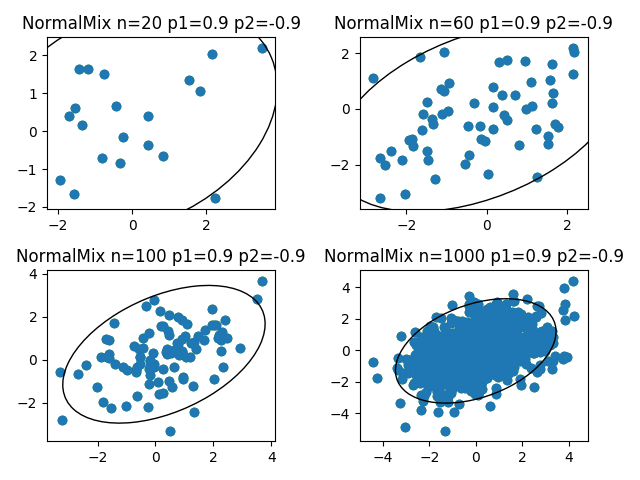
\includegraphics[scale = 0.6]{2p.png} 
    \label{fig:dis_norm_gis4}
\end{figure}
\begin{table}[H]
\caption{Результаты для смеси двумерных нормальных распределений}
\label{tab:my_label4}
\begin{center}
\vspace{5mm}
\begin{tabular}{|c|c|c|c|c|c|c|c|c|}
\hhline{----~----}
\multicolumn{4}{|c|}{NormalMix  $n=20,\;p_1 = 0.9,\;  p_2=-0.9$} &\multirow{11}{*}{$\cdot$} & \multicolumn{4}{c|} {NormalMix  $n=60,\; p_1 = -0.9,\;  p_2=-0.9$}
\\
\hhline{----~----}
&Pearson     &Spearman    &Quad &   & & Pearson     &Spearman    &Quad        \\    
\hhline{----~----}
		E   &0.33257&0.30331&0.18000&  &E   &0.41462&0.39782&0.21333\\
\hhline{----~----}
		$E^2$ &0.15235&0.12311&0.06000&  &$E^2$ &0.17848&0.16576&0.05422\\
\hhline{----~----}
		D   &0.04175&0.03111&0.02760&  &D   &0.00656&0.00749&0.00871\\\rowcolor{codegray}
\hhline{----~----} 
\multicolumn{9}{c}{}\\
\hhline{----~----}
\multicolumn{4}{|c|}{NormalMix  $n=100,\;p_1=0.9,\;  p_2=-0.9$} & & \multicolumn{4}{c|}{NormalMix  $n=1000,\;p_1=0.9,\;  p_2=-0.9$}\\
\hhline{----~----}
&Pearson     &Spearman    &Quad&  & &Pearson     &Spearman    &Quad     \\
\hhline{----~----}
		E   &0.42534&0.41706&0.31600& &E   &0.39241&0.37760&0.26000\\
\hhline{----~----}
		$E^2$ &0.18980&0.18042&0.10672& &$E^2$ &0.15440&0.14301&0.06812\\
\hhline{----~----}
		D   &0.00889&0.00648&0.00686& &D   &0.00042&0.00043&0.00052\\
\hhline{----~----}
\end{tabular}
\end{center}
\end{table}

\newpage
\section{Выводы}

По таблицам \ref{tab:my_label1}, \ref{tab:my_label2}, \ref{tab:my_label3}, \ref{tab:my_label4}, видно, что, при увеличении объёма выборки, подсчитанные коэффициенты корреляции стремятся к теоретическим.

Ближе всех к данному коэффициенту корреляции находится коэффициент Пирсона.

По графикам видно, что при уменьшении корреляции эллипс равновероятности стремится к окружности, а при увеличении растягивается.



\begin{thebibliography}{}
    \bibitem{numpy}  Модуль numpy  -  https://physics.susu.ru/vorontsov/language/numpy.html
    
    \bibitem{plotlib} 
    Модуль matplotlib - https://matplotlib.org/users/index.html
    
    \bibitem{skp}
    Модуль scipy - https://docs.scipy.org/doc/scipy/reference/
    
\bibitem{mix}
    http://stu.sernam.ru/book\_stat3.php?id=55
    
\bibitem{5_1}
Двумерное нормальное распределение: https://en.wikipedia.org/wiki/Multivariate\_normal\_distribution
\bibitem{5_2}
Коэффициент корреляции Пирса: http://statistica.ru/theory/koeffitsient-korrelyatsii/ 
\bibitem{5_3}
Коэффициент корреляции Спирмана: 
http://economic-definition.com/Exchange\_Terminology/Koefficient\_korrelyacii\_Correlation\_coefficient\_\_eto.html
\bibitem{5_4} Квадрантный коэффициент корреляции: https://www.researchgate.net/profile/Pavel\_Smirnov8/publication/\do-316973167\_Robastnye\_metody\_i\_algoritmy\_ocenivania\_korrelacionnyh\_harakteristik\_dannyh\_na\_os\do-nove\_novyh\_vysokoeffektivnyh\_i\_bystryh\_robastnyh\_ocenok\_masstaba/links/591b019d458515695282\do-8a52/Robastnye-metody-i-algoritmy-ocenivania-korrelacionnyh-harakteristik-dannyh-na-osnove-novyh-vysokoeffektivnyh-i-bystryh-robastnyh-ocenok-masstaba.pdf\#page=81

\end{thebibliography}


\section{Приложения}

Исходники: \url{https://github.com/LanskovNV/math_statistics/tree/master/lab_2}

\end{document}

